\hypertarget{efficiency-of-the-inference}{%
\section{Efficiency of the
inference}\label{efficiency-of-the-inference}}

\paragraph{Simulation settings}

For this simulation the data is simulated with
\(M = 2, n_{1}^{m} = 120, n_{2}^{m} = 120, Q_1 = Q_2 = 4\),
\(\bm{\alpha}, \bm{\pi}\) and \(\bm{\rho}\) are set as follows:
\begin{align*}
    &&\bm{\alpha} = .25 +
                    \begin{pmatrix}
                        3 \eps[\alpha] & 2 \eps[\alpha] & \eps[\alpha] & - \eps[\alpha]\\
                        2 \eps[\alpha] & 2 \eps[\alpha] & - \eps[\alpha] & \eps[\alpha]\\
                        \eps[\alpha] & - \eps[\alpha] & \eps[\alpha] & 2 \eps[\alpha]\\
                        - \eps[\alpha] & \eps[\alpha] & 2 \eps[\alpha] & 0
                    \end{pmatrix}, \\ \bm{\pi}^1 = \sigma_1
                    \begin{pmatrix}
                        0.2 & 0.4 & 0.4 & 0
                    \end{pmatrix},
                    && \bm{\pi}^2 =
                    \begin{pmatrix}
                        0.25 & 0.25 & 0.25 & 0.25
                    \end{pmatrix}, \\
                    \bm{\rho}^1 =
                    \begin{pmatrix}
                        0.25 & 0.25 & 0.25 & 0.25
                    \end{pmatrix}, &&
                    \bm{\rho}^2 = \sigma_2
                    \begin{pmatrix}
                        0 & 0.33 & 0.33 & 0.33
                    \end{pmatrix}, &&
\end{align*} with \(\eps[\alpha]\) taking nine equally spaced values
ranging from 0 to 0.24. For each value of \(\eps[\alpha]\), 108 datasets
(\(X_1, X_2\)) are simulated, resulting in \(9 \times 108 = 972\)
datasets. More precisely, for each dataset, we pick uniformly at random
two permutations of \(\{ 1, \dots , 4 \}\) (\(\sigma_1, \sigma_2\)) with
the constraint that \(\sigma_1(4) \neq \sigma_2(1)\). This ensures that
each of the two networks have a non-empty block that is empty in the
other one. Then the networks are simulated with
\(\mathcal{B}\)ern-\(BiSBM_{120}(4, \bm{\alpha}, \bm{\pi}^m, \bm{\rho}^m)\)
with the previous parameters. Each network has 2 blocks in common and
their connectivity structures encompass a mix of core-periphery,
assortative community and disassortative community structures, depending
on which 3 of the 4 blocks are selected for each network.
\(\eps[\alpha]\) represents the strength of these structures, the
larger, the easier it is to tell apart one block from another. The true
model of all the simulation is a \(\pi\rho\text{-}colBiSBM\).

\paragraph{Inference}

We want to measure the quality of the inference procedure, for this we
use the inference described in the section
\ref{sec:variational-estimation-of-the-parameters}.

\paragraph{Quality indicators}

To assess the quality of the inference, we will use the following
indicators:

\begin{itemize}
    \item First, for each dataset, we put in competition $\pi\text{-}colBiSBM$ with
    $sep\text{-}BiSBM$, $iid\text{-}colBiSBM$, $\rho\text{-}colBiSBM$,
    $\pi\rho\text{-}colBiSBM$
    respectively. To do so, for each dataset, we compute the
    BIC-L of each model $\pi\text{-}colBiSBM$ is preferred to $sep\text{-}BiSBM$
    (resp. $iid\text{-}colBiSBM$, $\rho\text{-}colBiSBM$,
    $\pi\rho\text{-}colBiSBM$) if
    its BIC-L is greater.
    \item When considering $\pi\text{-}colBiSBM$, $\rho\text{-}colBiSBM$,
    $\pi\rho\text{-}colBiSBM$ we compare $\widehat{Q_1}$, $\widehat{Q_2}$ to
    their true values. ($Q_1 = 4$ and $Q_2 = 4$)
    \item Finally, we assess the quality of the node grouping by computing the
    Adjusted Rand Index \parencite[][, ARI = 0 for a random grouping, ARI = 1 for a perfect recovery]{hubertComparingPartitions1985}. For each network, for the
    $\pi\text{-}colBiSBM$, $\rho\text{-}colBiSBM$,
    $\pi\rho\text{-}colBiSBM$ we compare the inferred block memberships to the
    real ones by computing the mean of the ARI per axis over the two networks
    \begin{equation*}
        \overline{\text{ARI}}_d = \frac{1}{2} \text{ARI}\big( \text{ARI}(\widehat{\bm{Z}^1_d},\bm{Z}^1_d) + \text{ARI}(\widehat{\bm{Z}^2_d},\bm{Z}^2_d) \big)
    \end{equation*}
    where $d$ is the dimension or axis (i.e., rows, $d=1$, or columns, $d=2$) of
    the block memberships.
    And we compute the ARI of the whole set of nodes to account for block
    pairing between networks
    \begin{equation*}
        \text{ARI}_d = \text{ARI}\big((\widehat{\bm{Z}^1_d},\widehat{\bm{Z}^2_d}),(\bm{Z}^1_d,\bm{Z}^2_d) \big)
    \end{equation*}
\end{itemize}

All these quality indicators are averaged over the 108 datasets. The
results are provided in the tables \ref{tab:per_model_sep} to
\ref{tab:per_model_pirho}. Each line corresponds to the 108 datasets for
a given value of value of \(\eps[\alpha]\).

\tiny
\begin{table}[!h]

\caption{\label{tab:per_model_table}\label{tab:per_model_sep}Quality metrics for $sep\text{-}BiSBM$}
\centering
\begin{tabular}[t]{rllll}
\toprule
$\eps[\alpha]$ & $\overline{\text{ARI}}_{1}$ & $\overline{\text{ARI}}_{2}$ & $\text{ARI}_{1}$ & $\text{ARI}_{2}$\\
\midrule
0.00 & 0 & 0 & 0 & 0\\
0.03 & 0 & 0 & 0 & 0\\
0.06 & 0.1 $\pm$ 0.01 & 0.08 $\pm$ 0.01 & 0.06 $\pm$ 0.01 & 0.05 $\pm$ 0.01\\
0.09 & 0.71 $\pm$ 0.02 & 0.7 $\pm$ 0.01 & 0.37 $\pm$ 0.02 & 0.37 $\pm$ 0.02\\
0.12 & 0.94 $\pm$ 0.01 & 0.93 $\pm$ 0.01 & 0.5 $\pm$ 0.02 & 0.49 $\pm$ 0.02\\
\addlinespace
0.15 & 0.99 & 0.99 & 0.54 $\pm$ 0.02 & 0.49 $\pm$ 0.01\\
0.18 & 0.99 & 0.99 & 0.52 $\pm$ 0.02 & 0.52 $\pm$ 0.02\\
0.21 & 0.99 & 0.99 & 0.54 $\pm$ 0.02 & 0.52 $\pm$ 0.02\\
0.24 & 1 & 1 & 0.55 $\pm$ 0.02 & 0.52 $\pm$ 0.02\\
\bottomrule
\end{tabular}
\end{table}
\begin{table}[!h]

\caption{\label{tab:per_model_table}\label{tab:per_model_iid}Quality metrics for $iid$$\text{-}colBiSBM$}
\centering
\begin{tabular}[t]{rllllll}
\toprule
$\eps[\alpha]$ & $\overline{\text{ARI}}_{1}$ & $\overline{\text{ARI}}_{2}$ & $\text{ARI}_{1}$ & $\text{ARI}_{2}$ & Recovered $Q_1$ & Recovered $Q_2$\\
\midrule
0.00 & 0 & 0 & 0 & 0 & 1 & 1\\
0.03 & 0 & 0 & 0 & 0 & 1 & 1\\
0.06 & 0.08 $\pm$ 0.01 & 0.08 $\pm$ 0.01 & 0.08 $\pm$ 0.01 & 0.07 $\pm$ 0.01 & 1.4 $\pm$ 0.05 & 1.49 $\pm$ 0.05\\
0.09 & 0.72 $\pm$ 0.01 & 0.71 $\pm$ 0.01 & 0.53 $\pm$ 0.02 & 0.52 $\pm$ 0.02 & 3.4 $\pm$ 0.06 & 3.41 $\pm$ 0.06\\
0.12 & 0.94 & 0.93 & 0.75 $\pm$ 0.03 & 0.72 $\pm$ 0.03 & 4.06 $\pm$ 0.02 & 3.97 $\pm$ 0.02\\
\addlinespace
0.15 & 0.98 & 0.98 & 0.77 $\pm$ 0.03 & 0.76 $\pm$ 0.03 & 4.11 $\pm$ 0.03 & 4.11 $\pm$ 0.03\\
0.18 & 0.99 & 0.99 & 0.82 $\pm$ 0.03 & 0.82 $\pm$ 0.03 & 4.15 $\pm$ 0.04 & 4.13 $\pm$ 0.03\\
0.21 & 0.99 & 0.99 & 0.8 $\pm$ 0.02 & 0.79 $\pm$ 0.03 & 4.35 $\pm$ 0.06 & 4.19 $\pm$ 0.04\\
0.24 & 0.99 & 0.99 & 0.77 $\pm$ 0.03 & 0.77 $\pm$ 0.03 & 4.3 $\pm$ 0.06 & 4.43 $\pm$ 0.07\\
\bottomrule
\end{tabular}
\end{table}
\begin{table}[!h]

\caption{\label{tab:per_model_table}\label{tab:per_model_pi}Quality metrics for $\pi$$\text{-}colBiSBM$}
\centering
\begin{tabular}[t]{rllllll}
\toprule
$\eps[\alpha]$ & $\overline{\text{ARI}}_{1}$ & $\overline{\text{ARI}}_{2}$ & $\text{ARI}_{1}$ & $\text{ARI}_{2}$ & Recovered $Q_1$ & Recovered $Q_2$\\
\midrule
0.00 & 0 & 0 & 0 & 0 & 1 & 1\\
0.03 & 0 & 0 & 0 & 0 & 1.01 $\pm$ 0.01 & 1\\
0.06 & 0.07 $\pm$ 0.01 & 0.08 $\pm$ 0.01 & 0.07 $\pm$ 0.01 & 0.06 $\pm$ 0.01 & 1.49 $\pm$ 0.05 & 1.5 $\pm$ 0.05\\
0.09 & 0.73 $\pm$ 0.02 & 0.72 $\pm$ 0.01 & 0.56 $\pm$ 0.02 & 0.53 $\pm$ 0.02 & 3.78 $\pm$ 0.07 & 3.37 $\pm$ 0.07\\
0.12 & 0.96 & 0.93 & 0.79 $\pm$ 0.02 & 0.74 $\pm$ 0.03 & 4.46 $\pm$ 0.07 & 3.95 $\pm$ 0.02\\
\addlinespace
0.15 & 0.99 & 0.97 & 0.82 $\pm$ 0.02 & 0.76 $\pm$ 0.03 & 4.62 $\pm$ 0.08 & 4\\
0.18 & 1 & 0.98 & 0.83 $\pm$ 0.02 & 0.79 $\pm$ 0.03 & 4.65 $\pm$ 0.09 & 4\\
0.21 & 1 & 0.98 & 0.84 $\pm$ 0.02 & 0.79 $\pm$ 0.03 & 4.69 $\pm$ 0.1 & 4\\
0.24 & 1 & 0.99 & 0.86 $\pm$ 0.02 & 0.79 $\pm$ 0.03 & 4.74 $\pm$ 0.11 & 4.01 $\pm$ 0.01\\
\bottomrule
\end{tabular}
\end{table}
\begin{table}[!h]

\caption{\label{tab:per_model_table}\label{tab:per_model_rho}Quality metrics for $\rho$$\text{-}colBiSBM$}
\centering
\begin{tabular}[t]{rllllll}
\toprule
$\eps[\alpha]$ & $\overline{\text{ARI}}_{1}$ & $\overline{\text{ARI}}_{2}$ & $\text{ARI}_{1}$ & $\text{ARI}_{2}$ & Recovered $Q_1$ & Recovered $Q_2$\\
\midrule
0.00 & 0 & 0 & 0 & 0 & 1 & 1\\
0.03 & 0 & 0 & 0 & 0 & 1.01 $\pm$ 0.01 & 1.01 $\pm$ 0.01\\
0.06 & 0.08 $\pm$ 0.01 & 0.08 $\pm$ 0.01 & 0.06 $\pm$ 0.01 & 0.07 $\pm$ 0.01 & 1.39 $\pm$ 0.05 & 1.6 $\pm$ 0.06\\
0.09 & 0.72 $\pm$ 0.01 & 0.72 $\pm$ 0.01 & 0.53 $\pm$ 0.02 & 0.54 $\pm$ 0.02 & 3.39 $\pm$ 0.07 & 3.74 $\pm$ 0.07\\
0.12 & 0.93 & 0.95 & 0.71 $\pm$ 0.03 & 0.75 $\pm$ 0.02 & 3.95 $\pm$ 0.02 & 4.5 $\pm$ 0.07\\
\addlinespace
0.15 & 0.97 & 0.99 & 0.78 $\pm$ 0.03 & 0.81 $\pm$ 0.02 & 4 & 4.49 $\pm$ 0.07\\
0.18 & 0.98 & 1 & 0.76 $\pm$ 0.03 & 0.81 $\pm$ 0.02 & 4.01 $\pm$ 0.01 & 4.71 $\pm$ 0.09\\
0.21 & 0.98 & 1 & 0.76 $\pm$ 0.03 & 0.81 $\pm$ 0.02 & 4.03 $\pm$ 0.02 & 4.72 $\pm$ 0.09\\
0.24 & 0.98 & 1 & 0.74 $\pm$ 0.03 & 0.8 $\pm$ 0.02 & 4.06 $\pm$ 0.02 & 4.8 $\pm$ 0.1\\
\bottomrule
\end{tabular}
\end{table}
\begin{table}[!h]

\caption{\label{tab:per_model_table}\label{tab:per_model_pirho}Quality metrics for $\pi\rho$$\text{-}colBiSBM$}
\centering
\begin{tabular}[t]{rllllll}
\toprule
$\eps[\alpha]$ & $\overline{\text{ARI}}_{1}$ & $\overline{\text{ARI}}_{2}$ & $\text{ARI}_{1}$ & $\text{ARI}_{2}$ & Recovered $Q_1$ & Recovered $Q_2$\\
\midrule
0.00 & 0 & 0 & 0 & 0 & 1 & 1\\
0.03 & 0 & 0 & 0 & 0 & 1.01 $\pm$ 0.01 & 1.01 $\pm$ 0.01\\
0.06 & 0.07 $\pm$ 0.01 & 0.07 $\pm$ 0.01 & 0.07 $\pm$ 0.01 & 0.06 $\pm$ 0.01 & 1.48 $\pm$ 0.05 & 1.57 $\pm$ 0.06\\
0.09 & 0.74 $\pm$ 0.01 & 0.73 $\pm$ 0.01 & 0.56 $\pm$ 0.03 & 0.55 $\pm$ 0.02 & 3.69 $\pm$ 0.06 & 3.66 $\pm$ 0.06\\
0.12 & 0.96 $\pm$ 0.01 & 0.95 $\pm$ 0.01 & 0.73 $\pm$ 0.03 & 0.73 $\pm$ 0.03 & 4.31 $\pm$ 0.05 & 4.26 $\pm$ 0.05\\
\addlinespace
0.15 & 0.99 & 0.99 & 0.79 $\pm$ 0.02 & 0.78 $\pm$ 0.03 & 4.31 $\pm$ 0.05 & 4.35 $\pm$ 0.05\\
0.18 & 1 & 1 & 0.83 $\pm$ 0.02 & 0.83 $\pm$ 0.02 & 4.31 $\pm$ 0.05 & 4.25 $\pm$ 0.04\\
0.21 & 1 & 1 & 0.77 $\pm$ 0.03 & 0.77 $\pm$ 0.03 & 4.42 $\pm$ 0.05 & 4.34 $\pm$ 0.05\\
0.24 & 1 & 1 & 0.82 $\pm$ 0.02 & 0.82 $\pm$ 0.02 & 4.25 $\pm$ 0.04 & 4.31 $\pm$ 0.05\\
\bottomrule
\end{tabular}
\end{table}
\normalsize

\begin{table}[!h]

\caption{\label{tab:proportion-preferred_model}\label{tab:proportion-preferred-table}Proportions of models selected per \eps[\alpha] (data for Figure \ref{fig:inference-proportion-preferred})}
\centering
\begin{tabular}[t]{rccccc}
\toprule
\eps[\alpha] & $sep\text{-}BiSBM$ & $iid\text{-}colBiSBM$ & $\pi\text{-}colBiSBM$ & $\rho\text{-}colBiSBM$ & $\pi\rho\text{-}colBiSBM$\\
\midrule
0.00 & 1.00 & 0.00 & 0.00 & 0.00 & 0.00\\
0.03 & 0.95 & 0.04 & 0.01 & 0.00 & 0.00\\
0.06 & 0.39 & 0.33 & 0.06 & 0.15 & 0.06\\
0.09 & 0.07 & 0.01 & 0.12 & 0.25 & 0.55\\
0.12 & 0.00 & 0.08 & 0.06 & 0.13 & 0.72\\
\addlinespace
0.15 & 0.00 & 0.12 & 0.08 & 0.08 & 0.71\\
0.18 & 0.00 & 0.11 & 0.04 & 0.06 & 0.79\\
0.21 & 0.00 & 0.19 & 0.04 & 0.07 & 0.69\\
0.24 & 0.00 & 0.09 & 0.06 & 0.08 & 0.77\\
\bottomrule
\end{tabular}
\end{table}

\begin{figure}
\centering
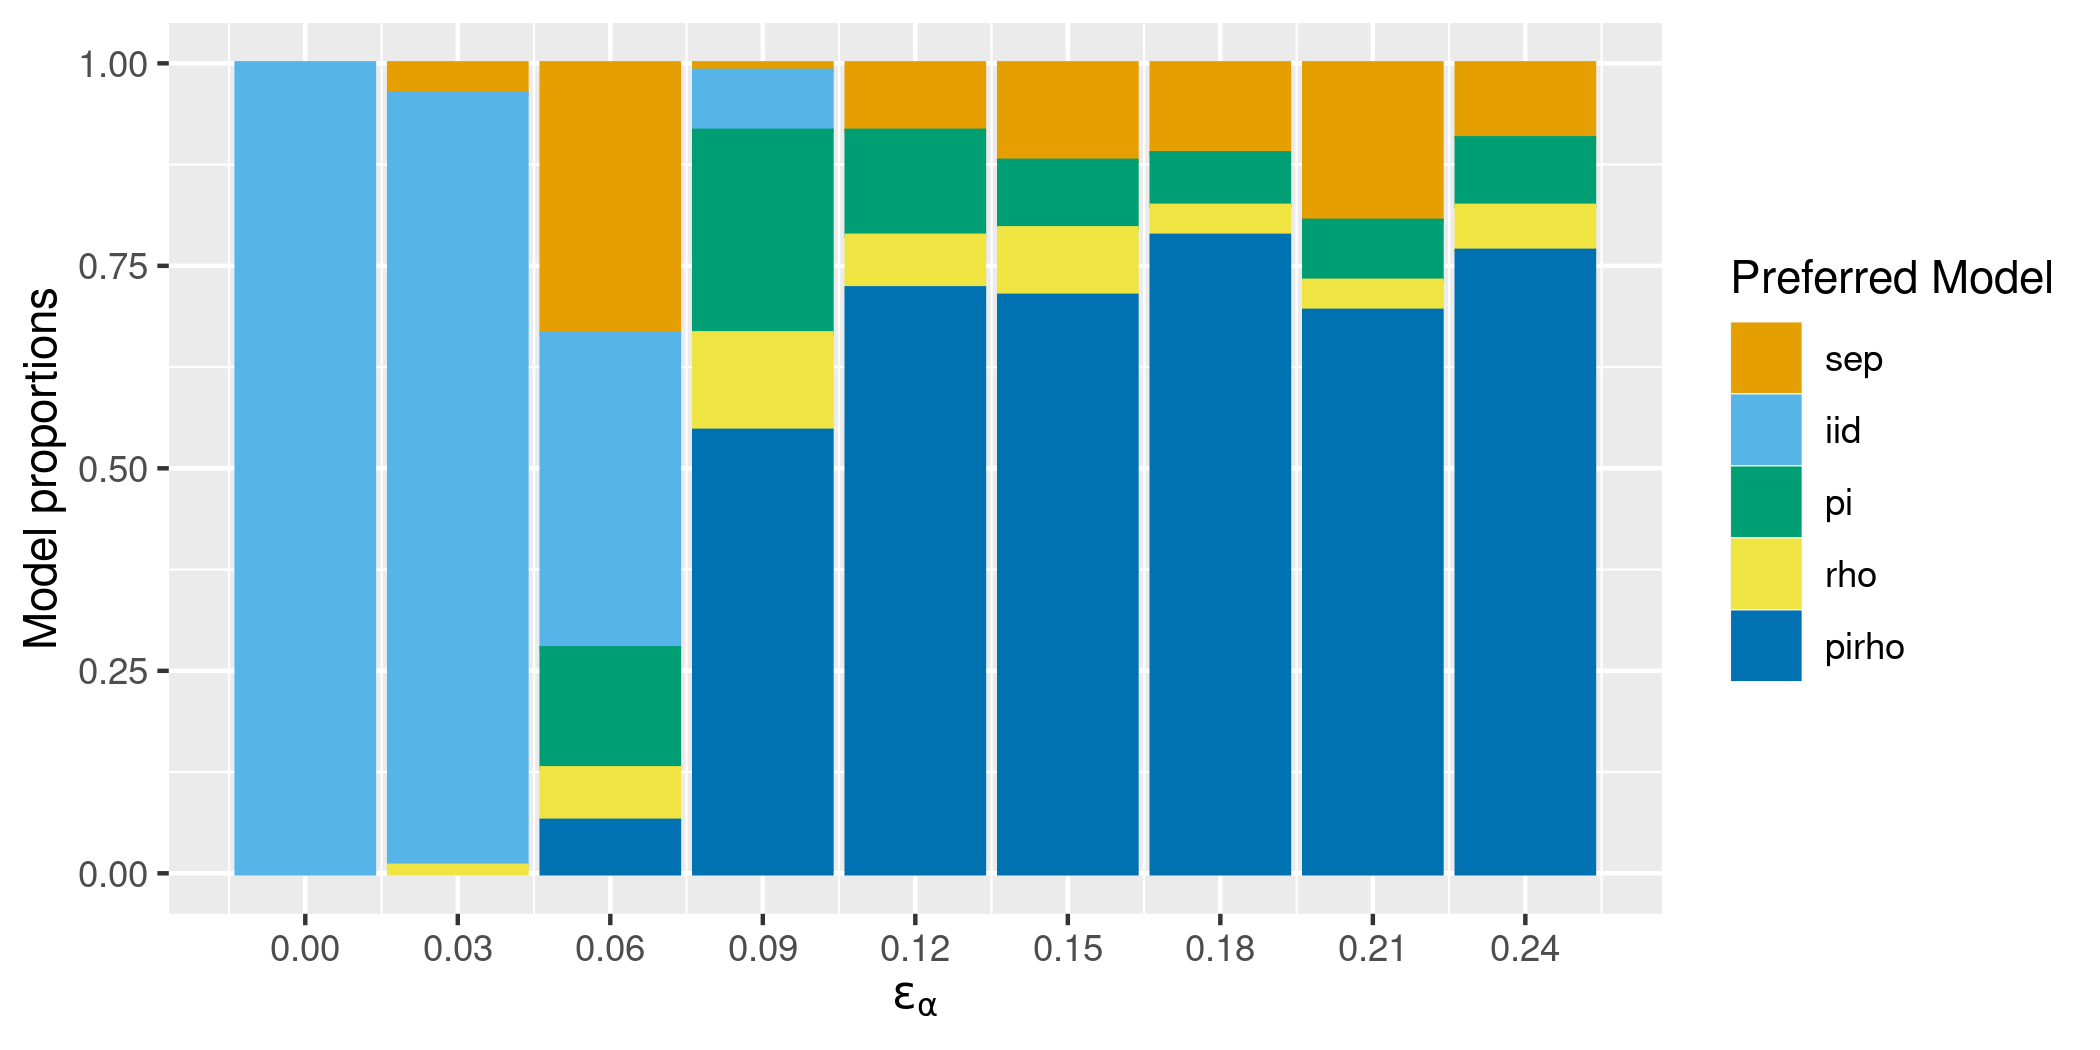
\includegraphics{./img/54eb0a21b143a53b6199a869d7a228ad7d158e57.png}
\caption{\label{fig:inference-proportion-preferred}Plot of the
proportions of different preferred models in function of \eps[\alpha]}
\end{figure}

\paragraph{Results}

For the model comparison, when \(\eps[\alpha]\) is small
(\(\eps[\alpha]\in[0, .04]\)), the simulation model is close to the
Erd\H{o}s-Reńyi network and it is very hard to find any structure beyond
the one of a single block on each dimension.

On the figure \ref{fig:inference-proportion-preferred} and table
\ref{tab:proportion-preferred-table} we can see that from
\(\eps[\alpha] = 0.12\) around \(70\%\) of the time the
\(\pi\rho\text{-}colBiSBM\) model (i.e., the correct one) is selected.

An interesting result we can read in the tables is that our models
outperform the \(sep\text{-}BiSBM\) when considering the ARI on the
whole set of nodes (\(\text{ARI}_d\)). This means that our models are
able to recover the block pairing \emph{between the networks} in
addition to recovering the blocks and their parameters.
